\documentclass[UTF8]{ctexart}
\usepackage{graphicx}
\graphicspath{{img/}} 
\title{Homework\ 5}
\author{PB17111623}
\author{PB17111623 范睿}
\date{\today}
\usepackage[a4paper,bottom=3.5cm]{geometry}
\usepackage{algorithm}  
\usepackage{algorithmicx}
\usepackage{amsmath}  
\usepackage{algpseudocode}  %算法的包
\usepackage{amssymb}
\begin{document}
\maketitle
\section{}
\subsection{考虑一个大小为 m = 1000 的散列表和一个对应的散列函数 $h(k) = \lfloor m(kA\ mod\ 1)\rfloor$,其中$A = (\sqrt{5} -  1)/2$,试计算关键字61,62,63,64和65被映射到的位置}
$h(61)=\lfloor 1000*(61*(\sqrt{5} -  1)/2\ mod\ 1)=700$\\
$h(62)=\lfloor 1000*(62*(\sqrt{5} -  1)/2\ mod\ 1)=318$\\
$h(63)=\lfloor 1000*(63*(\sqrt{5} -  1)/2\ mod\ 1)=936$\\
$h(64)=\lfloor 1000*(64*(\sqrt{5} -  1)/2\ mod\ 1)=554$\\
$h(65)=\lfloor 1000*(65*(\sqrt{5} -  1)/2\ mod\ 1)=172$

\subsection{考虑用开放寻址法将关键字 10,22,31,4,15,28,17,88,59 插入到一长度为 $m = 11$ 的散列表中,辅助散列函数为$h'(k) = k$。试说明分别用线性探查、二次探查$(c1 = 1, c2 = 3)$和双重散列$(h1(k) = k,h2(k) = 1+(k\ mod\ (m - 1)))$将这些关键字插入散列表的过程。}
\subsubsection{线性探查}
10:$\ h'(10)=10,\ T[10]=10$\\
22:$\ h'(22)=0,\ T[0]=22$\\
31:$\ h'(31)=9,\ T[9]=31$\\
4:$\ \ h'(4)=4,\ T[4]=4$\\
15:$\ h'(15)=4,h(15,1)=5,\ T[5]=15$\\
28:$\ h'(28)=6,\ T[6]=28$\\
17:$\ h'(17)=6,h(17,1)=7,\ T[7]=17$\\
88:$\ h'(88)=0,h(88,1)=1,\ T[1]=88$\\
59:$\ h'(59)=4, h(59,1)=5, h(59,2)=6, h(59,3)=7, h(59,4)=8\ T[8]=59$
\subsubsection{二次探查}
10:$\ h'(10)=10,\ T[10]=10$\\
22:$\ h'(22)=0,\ T[0]=22$\\
31:$\ h'(31)=9,\ T[9]=31$\\
4:$\ \ h'(4)=4,\ T[4]=4$\\
15:$\ h'(15)=4,h(15,1)=8,\ T[8]=15$\\
28:$\ h'(28)=6,\ T[6]=28$\\
17:$\ h'(17)=6,h(17,1)=10,h(17,2)=9, h(17,3)=3\ T[3]=17$\\
88:$\ h'(88)=0,h(88,1)=4,h(88,2)=3,h(88,3)=8,h(88,4)=8,h(88,5)=3,h(88,6)=4,h(88,7)=0,h(88,8)=2\ T[2]=88$\\
59:$\ h'(59)=4, h(59,1)=8,h(59,2)=7,\ T[7]=59$
\subsubsection{双重散列}
10:$\ h'(10)=10,\ T[10]=10$\\
22:$\ h'(22)=0,\ T[0]=22$\\
31:$\ h'(31)=9,\ T[9]=31$\\
4:$\ \ h'(4)=4,\ T[4]=4$\\
15:$\ h'(15)=4,h(15,1)=10,h(15,2)=5\ T[5]=15$\\
28:$\ h'(28)=6,\ T[6]=28$\\
17:$\ h'(17)=6,h(17,1)=3,\ T[3]=17$\\
88:$\ h'(88)=0,h(88,1)=9,h(88,2)=7\ T[7]=88$\\
59:$\ h'(59)=4, h(59,1)=3,h(59,2)=2\ T[2]=59$
\subsection{因为在基于比较的排序模型中,完成$n$个元素的排序,其最坏情况下需要 $\Omega(n\lg n)$ 时间。试证明:任何基于比较的算法从$n$个元素的任意序列中构造一棵二叉搜索树,其最坏情况下需要 $\Omega(n\lg n)$ 的时间}
证明:\\
由于一颗二叉搜索树的中序排列是此树中所有元素从小到大的排列,因此将一组无序数列构造成一棵二叉搜索树等同于将它们从小到大排列。由于任何基于比较的排序模型将n个数完成排序的时间为$\Omega(n\lg n)$,因此利用基于比较的算法构造一棵二叉搜索树的时间也为$\Omega(n\lg n)$
\subsubsection{将关键字 41,38,31,12,19,8 连续地插入一棵初始为空的红黑树之后,试画出该结果树}
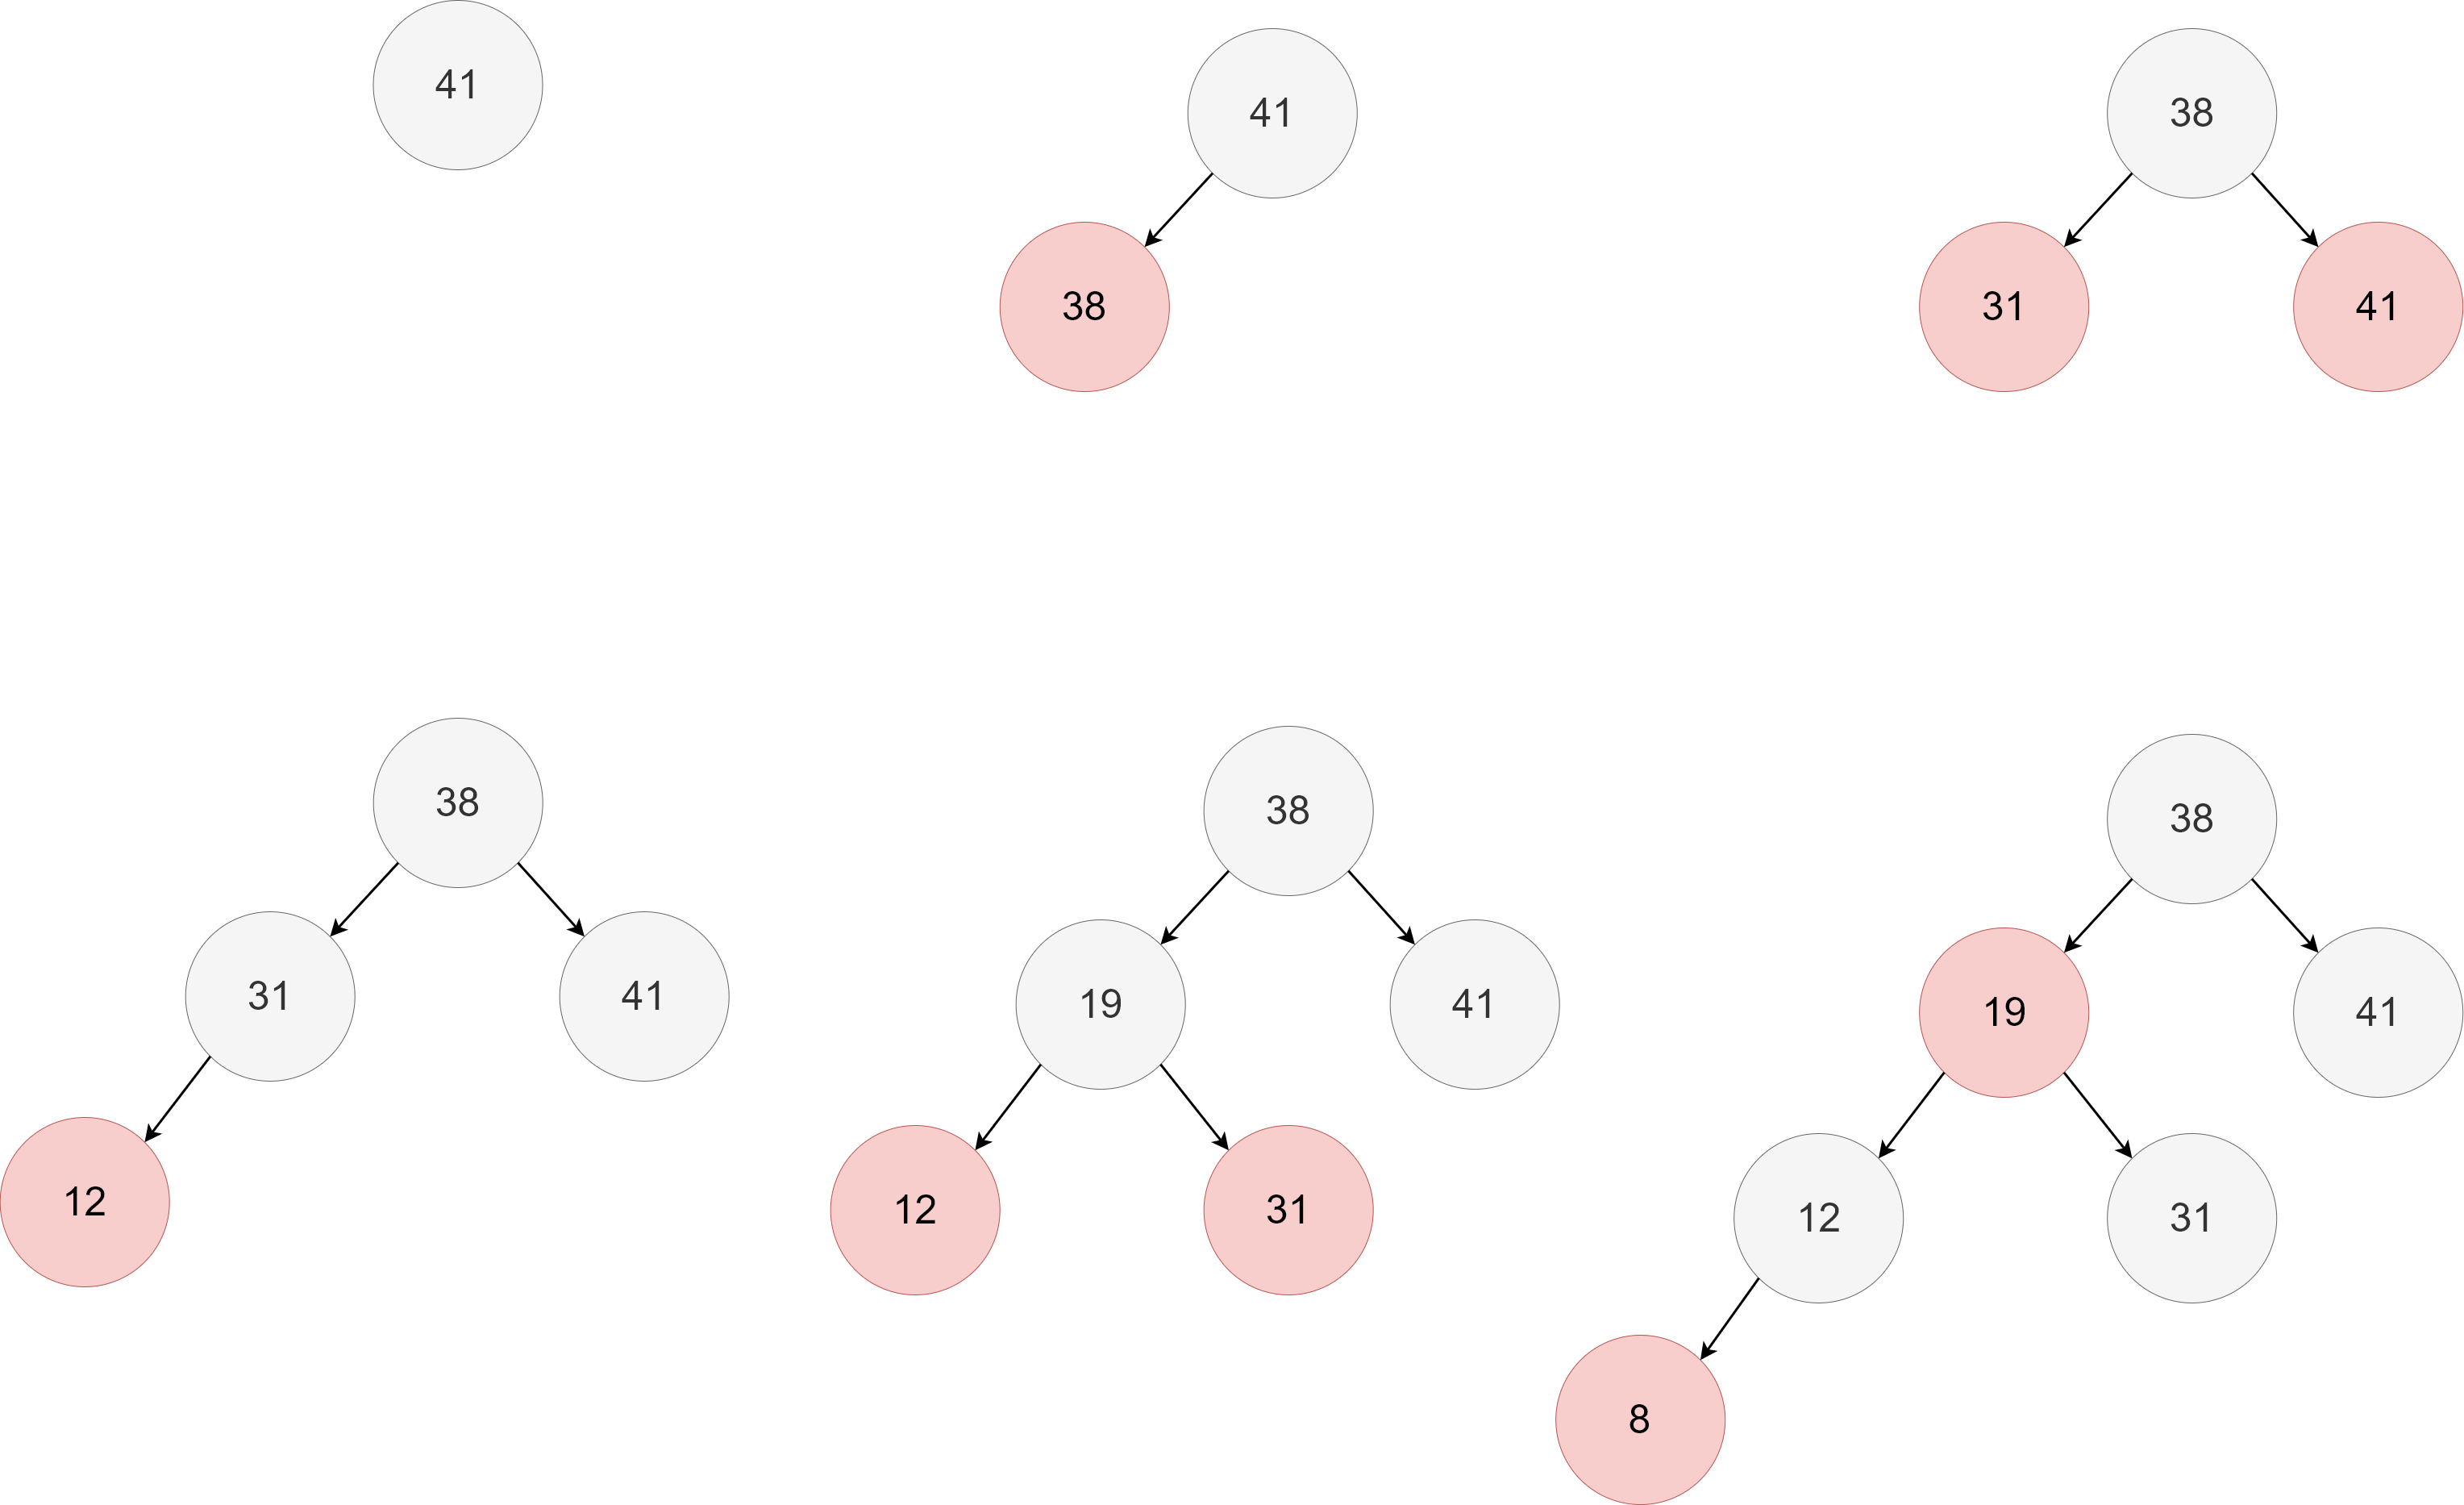
\includegraphics[scale=0.11]{img/4.png}
\subsubsection{对于1中得到的红黑树,依次删除 8,12,19,试画出每次删除操作后的红黑树}
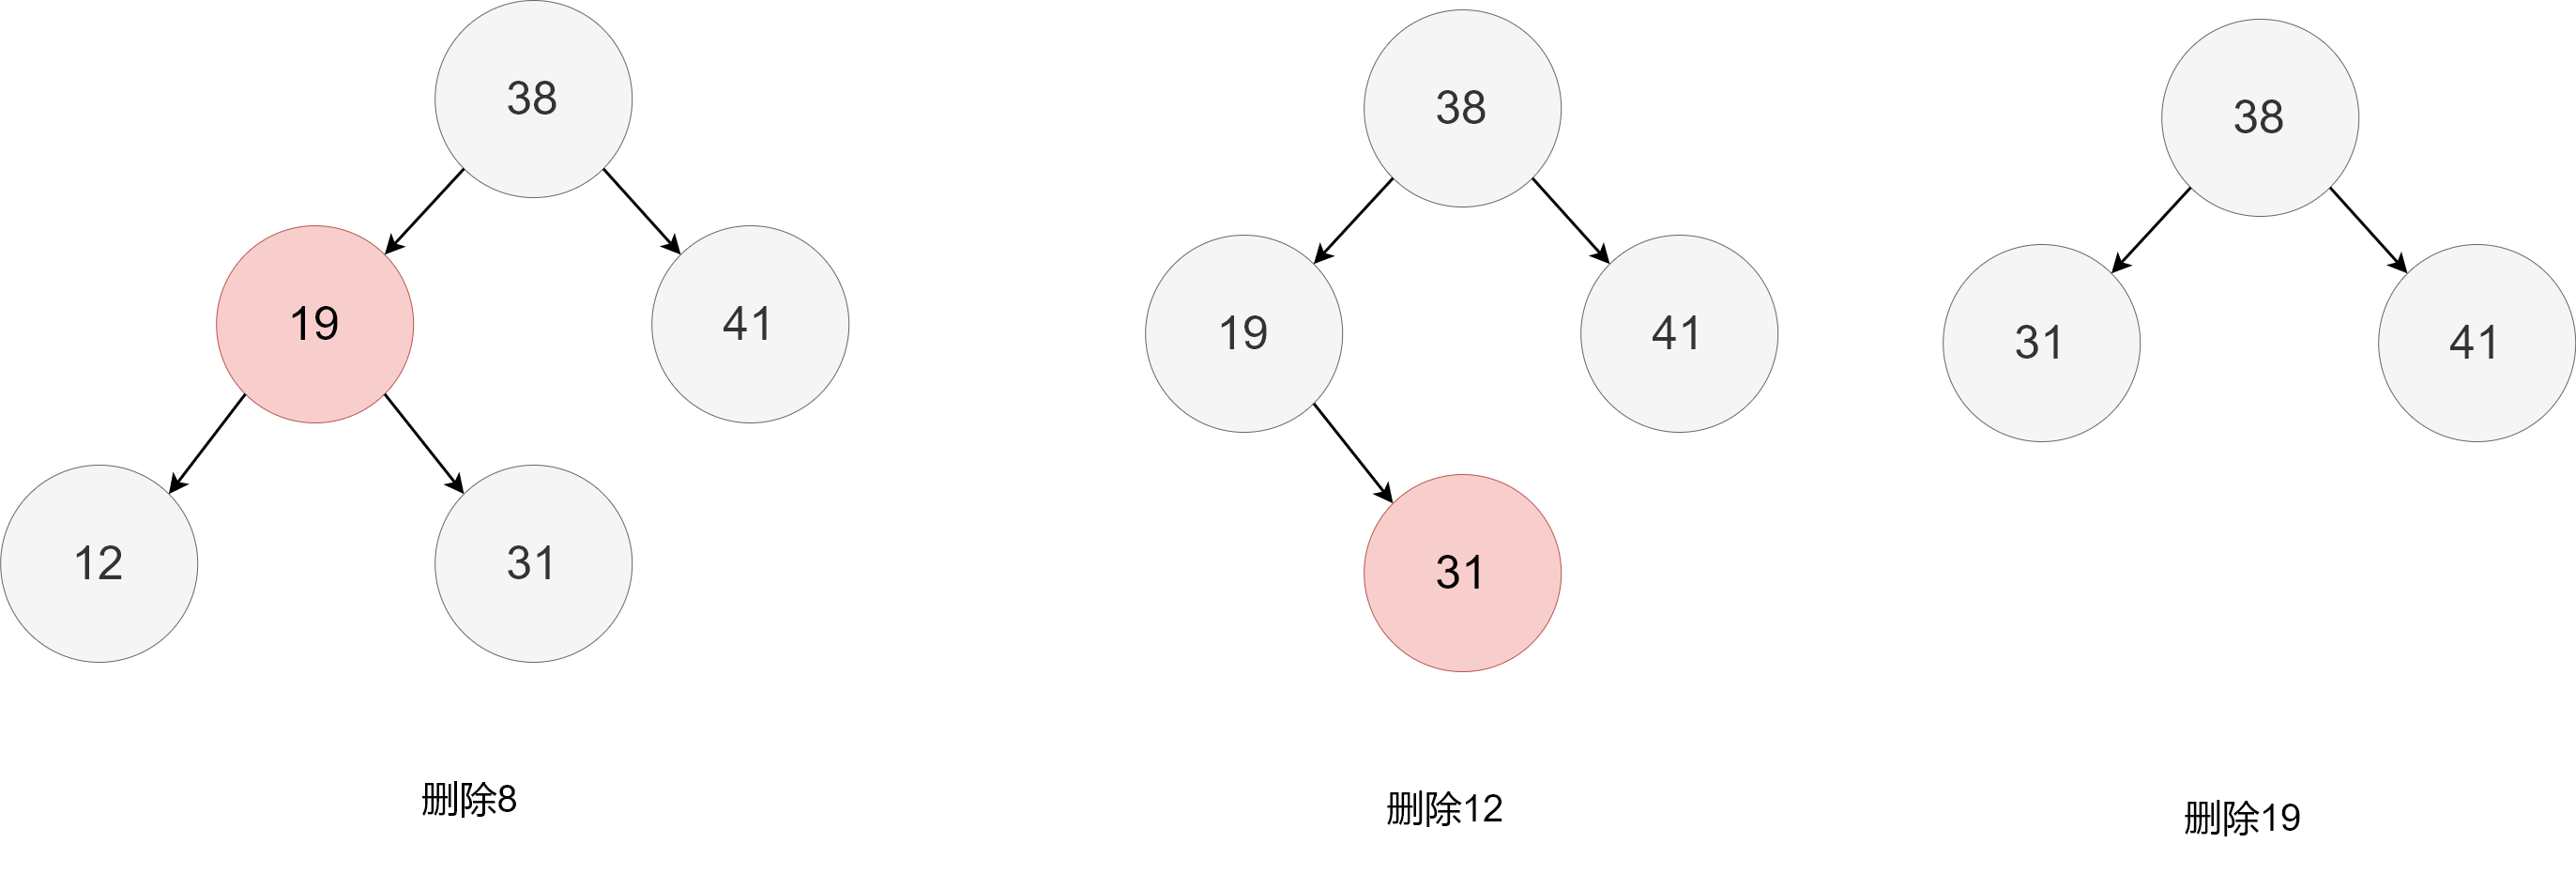
\includegraphics[scale=0.13]{img/4_1.png}
\end{document}

















